% Created by tikzDevice version 0.12.6 on 2024-05-31 23:46:11
% !TEX encoding = UTF-8 Unicode
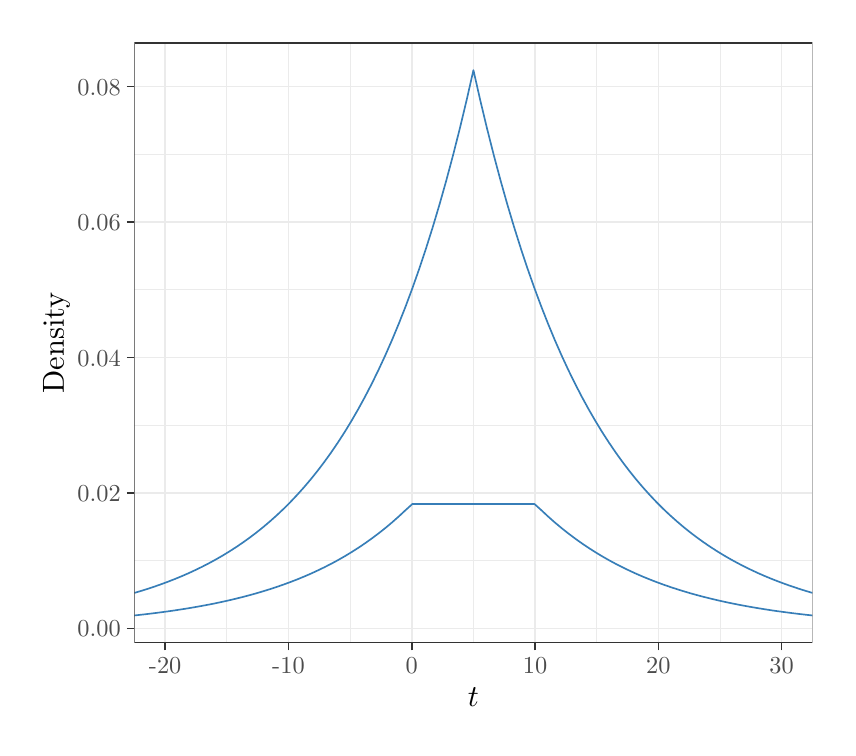
\begin{tikzpicture}[x=1pt,y=1pt]
\definecolor{fillColor}{RGB}{255,255,255}
\path[use as bounding box,fill=fillColor,fill opacity=0.00] (0,0) rectangle (289.08,252.94);
\begin{scope}
\path[clip] (  0.00,  0.00) rectangle (289.08,252.94);
\definecolor{drawColor}{RGB}{255,255,255}
\definecolor{fillColor}{RGB}{255,255,255}

\path[draw=drawColor,line width= 0.6pt,line join=round,line cap=round,fill=fillColor] (  0.00,  0.00) rectangle (289.08,252.94);
\end{scope}
\begin{scope}
\path[clip] ( 38.56, 30.69) rectangle (283.58,247.45);
\definecolor{fillColor}{RGB}{255,255,255}

\path[fill=fillColor] ( 38.56, 30.69) rectangle (283.58,247.45);
\definecolor{drawColor}{gray}{0.92}

\path[draw=drawColor,line width= 0.3pt,line join=round] ( 38.56, 60.27) --
	(283.58, 60.27);

\path[draw=drawColor,line width= 0.3pt,line join=round] ( 38.56,109.23) --
	(283.58,109.23);

\path[draw=drawColor,line width= 0.3pt,line join=round] ( 38.56,158.19) --
	(283.58,158.19);

\path[draw=drawColor,line width= 0.3pt,line join=round] ( 38.56,207.15) --
	(283.58,207.15);

\path[draw=drawColor,line width= 0.3pt,line join=round] ( 71.97, 30.69) --
	( 71.97,247.45);

\path[draw=drawColor,line width= 0.3pt,line join=round] (116.52, 30.69) --
	(116.52,247.45);

\path[draw=drawColor,line width= 0.3pt,line join=round] (161.07, 30.69) --
	(161.07,247.45);

\path[draw=drawColor,line width= 0.3pt,line join=round] (205.62, 30.69) --
	(205.62,247.45);

\path[draw=drawColor,line width= 0.3pt,line join=round] (250.17, 30.69) --
	(250.17,247.45);

\path[draw=drawColor,line width= 0.6pt,line join=round] ( 38.56, 35.79) --
	(283.58, 35.79);

\path[draw=drawColor,line width= 0.6pt,line join=round] ( 38.56, 84.75) --
	(283.58, 84.75);

\path[draw=drawColor,line width= 0.6pt,line join=round] ( 38.56,133.71) --
	(283.58,133.71);

\path[draw=drawColor,line width= 0.6pt,line join=round] ( 38.56,182.67) --
	(283.58,182.67);

\path[draw=drawColor,line width= 0.6pt,line join=round] ( 38.56,231.63) --
	(283.58,231.63);

\path[draw=drawColor,line width= 0.6pt,line join=round] ( 49.69, 30.69) --
	( 49.69,247.45);

\path[draw=drawColor,line width= 0.6pt,line join=round] ( 94.24, 30.69) --
	( 94.24,247.45);

\path[draw=drawColor,line width= 0.6pt,line join=round] (138.79, 30.69) --
	(138.79,247.45);

\path[draw=drawColor,line width= 0.6pt,line join=round] (183.34, 30.69) --
	(183.34,247.45);

\path[draw=drawColor,line width= 0.6pt,line join=round] (227.89, 30.69) --
	(227.89,247.45);

\path[draw=drawColor,line width= 0.6pt,line join=round] (272.44, 30.69) --
	(272.44,247.45);
\definecolor{drawColor}{RGB}{55,126,184}

\path[draw=drawColor,line width= 0.6pt,line join=round] ( 38.56, 40.54) --
	( 41.01, 40.81) --
	( 43.46, 41.09) --
	( 45.91, 41.39) --
	( 48.36, 41.71) --
	( 50.81, 42.04) --
	( 53.26, 42.39) --
	( 55.71, 42.77) --
	( 58.16, 43.16) --
	( 60.61, 43.58) --
	( 63.06, 44.02) --
	( 65.51, 44.48) --
	( 67.96, 44.97) --
	( 70.41, 45.49) --
	( 72.86, 46.04) --
	( 75.31, 46.62) --
	( 77.76, 47.23) --
	( 80.21, 47.88) --
	( 82.66, 48.56) --
	( 85.11, 49.29) --
	( 87.56, 50.05) --
	( 90.01, 50.86) --
	( 92.46, 51.71) --
	( 94.91, 52.61) --
	( 97.36, 53.56) --
	( 99.81, 54.56) --
	(102.26, 55.62) --
	(104.71, 56.75) --
	(107.16, 57.93) --
	(109.61, 59.18) --
	(112.06, 60.50) --
	(114.51, 61.90) --
	(116.96, 63.38) --
	(119.41, 64.94) --
	(121.86, 66.59) --
	(124.31, 68.33) --
	(126.76, 70.17) --
	(129.21, 72.11) --
	(131.66, 74.16) --
	(134.11, 76.33) --
	(136.57, 78.62) --
	(139.02, 80.82) --
	(141.47, 80.82) --
	(143.92, 80.82) --
	(146.37, 80.82) --
	(148.82, 80.82) --
	(151.27, 80.82) --
	(153.72, 80.82) --
	(156.17, 80.82) --
	(158.62, 80.82) --
	(161.07, 80.82) --
	(163.52, 80.82) --
	(165.97, 80.82) --
	(168.42, 80.82) --
	(170.87, 80.82) --
	(173.32, 80.82) --
	(175.77, 80.82) --
	(178.22, 80.82) --
	(180.67, 80.82) --
	(183.12, 80.82) --
	(185.57, 78.62) --
	(188.02, 76.33) --
	(190.47, 74.16) --
	(192.92, 72.11) --
	(195.37, 70.17) --
	(197.82, 68.33) --
	(200.27, 66.59) --
	(202.72, 64.94) --
	(205.17, 63.38) --
	(207.62, 61.90) --
	(210.07, 60.50) --
	(212.52, 59.18) --
	(214.97, 57.93) --
	(217.42, 56.75) --
	(219.87, 55.62) --
	(222.32, 54.56) --
	(224.77, 53.56) --
	(227.22, 52.61) --
	(229.67, 51.71) --
	(232.12, 50.86) --
	(234.58, 50.05) --
	(237.03, 49.29) --
	(239.48, 48.56) --
	(241.93, 47.88) --
	(244.38, 47.23) --
	(246.83, 46.62) --
	(249.28, 46.04) --
	(251.73, 45.49) --
	(254.18, 44.97) --
	(256.63, 44.48) --
	(259.08, 44.02) --
	(261.53, 43.58) --
	(263.98, 43.16) --
	(266.43, 42.77) --
	(268.88, 42.39) --
	(271.33, 42.04) --
	(273.78, 41.71) --
	(276.23, 41.39) --
	(278.68, 41.09) --
	(281.13, 40.81) --
	(283.58, 40.54);

\path[draw=drawColor,line width= 0.6pt,line join=round] ( 38.56, 48.69) --
	( 41.01, 49.42) --
	( 43.46, 50.19) --
	( 45.91, 51.01) --
	( 48.36, 51.87) --
	( 50.81, 52.78) --
	( 53.26, 53.74) --
	( 55.71, 54.75) --
	( 58.16, 55.82) --
	( 60.61, 56.96) --
	( 63.06, 58.15) --
	( 65.51, 59.42) --
	( 67.96, 60.75) --
	( 70.41, 62.16) --
	( 72.86, 63.65) --
	( 75.31, 65.23) --
	( 77.76, 66.89) --
	( 80.21, 68.65) --
	( 82.66, 70.51) --
	( 85.11, 72.47) --
	( 87.56, 74.55) --
	( 90.01, 76.74) --
	( 92.46, 79.05) --
	( 94.91, 81.50) --
	( 97.36, 84.09) --
	( 99.81, 86.82) --
	(102.26, 89.70) --
	(104.71, 92.75) --
	(107.16, 95.97) --
	(109.61, 99.37) --
	(112.06,102.97) --
	(114.51,106.76) --
	(116.96,110.78) --
	(119.41,115.02) --
	(121.86,119.50) --
	(124.31,124.23) --
	(126.76,129.23) --
	(129.21,134.51) --
	(131.66,140.09) --
	(134.11,145.99) --
	(136.57,152.22) --
	(139.02,158.80) --
	(141.47,165.76) --
	(143.92,173.11) --
	(146.37,180.87) --
	(148.82,189.07) --
	(151.27,197.74) --
	(153.72,206.90) --
	(156.17,216.57) --
	(158.62,226.79) --
	(161.07,237.59) --
	(163.52,226.79) --
	(165.97,216.57) --
	(168.42,206.90) --
	(170.87,197.74) --
	(173.32,189.07) --
	(175.77,180.87) --
	(178.22,173.11) --
	(180.67,165.76) --
	(183.12,158.80) --
	(185.57,152.22) --
	(188.02,145.99) --
	(190.47,140.09) --
	(192.92,134.51) --
	(195.37,129.23) --
	(197.82,124.23) --
	(200.27,119.50) --
	(202.72,115.02) --
	(205.17,110.78) --
	(207.62,106.76) --
	(210.07,102.97) --
	(212.52, 99.37) --
	(214.97, 95.97) --
	(217.42, 92.75) --
	(219.87, 89.70) --
	(222.32, 86.82) --
	(224.77, 84.09) --
	(227.22, 81.50) --
	(229.67, 79.05) --
	(232.12, 76.74) --
	(234.58, 74.55) --
	(237.03, 72.47) --
	(239.48, 70.51) --
	(241.93, 68.65) --
	(244.38, 66.89) --
	(246.83, 65.23) --
	(249.28, 63.65) --
	(251.73, 62.16) --
	(254.18, 60.75) --
	(256.63, 59.42) --
	(259.08, 58.15) --
	(261.53, 56.96) --
	(263.98, 55.82) --
	(266.43, 54.75) --
	(268.88, 53.74) --
	(271.33, 52.78) --
	(273.78, 51.87) --
	(276.23, 51.01) --
	(278.68, 50.19) --
	(281.13, 49.42) --
	(283.58, 48.69);
\definecolor{drawColor}{gray}{0.20}

\path[draw=drawColor,line width= 0.6pt,line join=round,line cap=round] ( 38.56, 30.69) rectangle (283.58,247.45);
\end{scope}
\begin{scope}
\path[clip] (  0.00,  0.00) rectangle (289.08,252.94);
\definecolor{drawColor}{gray}{0.30}

\node[text=drawColor,anchor=base east,inner sep=0pt, outer sep=0pt, scale=  0.88] at ( 33.61, 32.76) {0.00};

\node[text=drawColor,anchor=base east,inner sep=0pt, outer sep=0pt, scale=  0.88] at ( 33.61, 81.72) {0.02};

\node[text=drawColor,anchor=base east,inner sep=0pt, outer sep=0pt, scale=  0.88] at ( 33.61,130.68) {0.04};

\node[text=drawColor,anchor=base east,inner sep=0pt, outer sep=0pt, scale=  0.88] at ( 33.61,179.64) {0.06};

\node[text=drawColor,anchor=base east,inner sep=0pt, outer sep=0pt, scale=  0.88] at ( 33.61,228.60) {0.08};
\end{scope}
\begin{scope}
\path[clip] (  0.00,  0.00) rectangle (289.08,252.94);
\definecolor{drawColor}{gray}{0.20}

\path[draw=drawColor,line width= 0.6pt,line join=round] ( 35.81, 35.79) --
	( 38.56, 35.79);

\path[draw=drawColor,line width= 0.6pt,line join=round] ( 35.81, 84.75) --
	( 38.56, 84.75);

\path[draw=drawColor,line width= 0.6pt,line join=round] ( 35.81,133.71) --
	( 38.56,133.71);

\path[draw=drawColor,line width= 0.6pt,line join=round] ( 35.81,182.67) --
	( 38.56,182.67);

\path[draw=drawColor,line width= 0.6pt,line join=round] ( 35.81,231.63) --
	( 38.56,231.63);
\end{scope}
\begin{scope}
\path[clip] (  0.00,  0.00) rectangle (289.08,252.94);
\definecolor{drawColor}{gray}{0.20}

\path[draw=drawColor,line width= 0.6pt,line join=round] ( 49.69, 27.94) --
	( 49.69, 30.69);

\path[draw=drawColor,line width= 0.6pt,line join=round] ( 94.24, 27.94) --
	( 94.24, 30.69);

\path[draw=drawColor,line width= 0.6pt,line join=round] (138.79, 27.94) --
	(138.79, 30.69);

\path[draw=drawColor,line width= 0.6pt,line join=round] (183.34, 27.94) --
	(183.34, 30.69);

\path[draw=drawColor,line width= 0.6pt,line join=round] (227.89, 27.94) --
	(227.89, 30.69);

\path[draw=drawColor,line width= 0.6pt,line join=round] (272.44, 27.94) --
	(272.44, 30.69);
\end{scope}
\begin{scope}
\path[clip] (  0.00,  0.00) rectangle (289.08,252.94);
\definecolor{drawColor}{gray}{0.30}

\node[text=drawColor,anchor=base,inner sep=0pt, outer sep=0pt, scale=  0.88] at ( 49.69, 19.68) {-20};

\node[text=drawColor,anchor=base,inner sep=0pt, outer sep=0pt, scale=  0.88] at ( 94.24, 19.68) {-10};

\node[text=drawColor,anchor=base,inner sep=0pt, outer sep=0pt, scale=  0.88] at (138.79, 19.68) {0};

\node[text=drawColor,anchor=base,inner sep=0pt, outer sep=0pt, scale=  0.88] at (183.34, 19.68) {10};

\node[text=drawColor,anchor=base,inner sep=0pt, outer sep=0pt, scale=  0.88] at (227.89, 19.68) {20};

\node[text=drawColor,anchor=base,inner sep=0pt, outer sep=0pt, scale=  0.88] at (272.44, 19.68) {30};
\end{scope}
\begin{scope}
\path[clip] (  0.00,  0.00) rectangle (289.08,252.94);
\definecolor{drawColor}{RGB}{0,0,0}

\node[text=drawColor,anchor=base,inner sep=0pt, outer sep=0pt, scale=  1.10] at (161.07,  7.64) {$t$};
\end{scope}
\begin{scope}
\path[clip] (  0.00,  0.00) rectangle (289.08,252.94);
\definecolor{drawColor}{RGB}{0,0,0}

\node[text=drawColor,rotate= 90.00,anchor=base,inner sep=0pt, outer sep=0pt, scale=  1.10] at ( 13.08,139.07) {Density};
\end{scope}
\end{tikzpicture}
